\begin{center}
    \begin{tabular}{c c}
        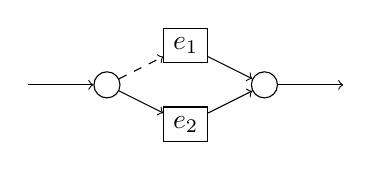
\begin{tikzpicture}
            \node[circle, draw] (start) at (0, 0) {};
            \node[draw] (e1) at (1, 0.5) {$e_1$};
            \node[draw] (e2) at (1, -0.5) {$e_2$};
            \node[circle, draw] (end) at (2, 0) {};
            
            \draw[->] (-1, 0) -- (start);
            \draw[->, dashed] (start) -- (e1); \draw[->] (e1) -- (end);
            \draw[->] (start) -- (e2); \draw[->] (e2) -- (end);
            \draw[->] (end) -- (3, 0);
        \end{tikzpicture} & 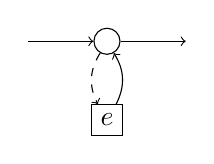
\begin{tikzpicture}
            \node[draw] (e) at (0, 0) {$e$};
            \node[draw, circle] (root) at (0, 1) {};
            
            \draw[->] (-1, 1) -- (root);
            \draw[->] (root) -- (1, 1);
            \draw[->, dashed] (root) to[bend right] (e);
            \draw[->] (e) to[bend right] (root);
        \end{tikzpicture}
    \end{tabular} \\ \vspace{0.3ex}
    \textit{NFA constructions for $e_1 \ | \ e_2$ and $e^*$} \\
    \textit{Dashed edges are higher priority edges.}
\end{center}